%%%%%%%%%%%%%%%%%%%%%%%%%%%%%%%%%%%%%%%%%%%%%%%%%%%%%%%%%%%%%%%%%%%%%%%%%%%%%%%%
%%%%%%%%%%%%%%%%%%%%%%%%%%%%%%%%%%%%%%%%%%%%%%%%%%%%%%%%%%%%%%%%%%%%%%%%%%%%%%%%
%\documentclass[addpoints,12pt,solution]{exam}
\documentclass[preprint,12pt]{elsarticle}
%% Use the option review to obtain double line spacing

%% Use the options 1p,twocolumn; 3p; 3p,twocolumn; 5p; or 5p,twocolumn
%% for a journal layout:
%% \documentclass[final,1p,times]{elsarticle}
%% \documentclass[final,1p,times,twocolumn]{elsarticle}
%% \documentclass[final,3p,times]{elsarticle}
%% \documentclass[final,3p,times,twocolumn]{elsarticle}
%% \documentclass[final,5p,times]{elsarticle}
%% \documentclass[final,5p,times,twocolumn]{elsarticle}

%% The graphicx package provides the includegraphics command.
\usepackage{graphicx}
%% The amssymb package provides various useful mathematical symbols
\usepackage{amssymb}
\usepackage{amsmath}
\usepackage{breqn}
\usepackage{chemfig}
\usepackage{csvsimple}
%% The amsthm package provides extended theorem environments
%% \usepackage{amsthm}

%% The lineno packages adds line numbers. Start line numbering with
%% \begin{linenumbers}, end it with \end{linenumbers}. Or switch it on
%% for the whole article with \linenumbers after \end{frontmatter}.
\usepackage{lineno}
\usepackage{natbib}
\usepackage{hyperref}
% \usepackage[top=0.75in, bottom=0.75in, left=0.55in, right=0.85in]{geometry}
\usepackage{graphicx}
\usepackage{url}
\usepackage{palatino}
\usepackage{tabularx}
\usepackage{graphicx}
\usepackage{multicol}
\usepackage{graphicx}
\usepackage{amssymb}
\usepackage{float}
\usepackage{amsmath}
\usepackage{rotating}
\usepackage{subfigure}
\usepackage{multirow}
\usepackage{mathrsfs}
\usepackage{xfrac}
\usepackage[font=small,skip=0pt]{caption}
%\usepackage[numbers,sort&compress]{natbib}
%\usepackage{hyperref}
\usepackage{pgf,tikz}
\usetikzlibrary{shapes,arrows,chains}
\usetikzlibrary[calc]
\usepackage{graphicx}
\graphicspath{ {./images/},{./images/Q1},{./images/Q2}}
\usepackage{geometry}
\geometry{lmargin=1in,rmargin=1in,tmargin=1in,bmargin=1in}
\usepackage{lipsum}
%\pagestyle{empty}
\usepackage{natbib}
\pagenumbering{arabic}
%\usepackage[T1]{fontenc}
\usepackage{setspace}
\usepackage{mathptmx}
\usepackage{t1enc}
%\usepackage{xkeyval}
%\usepackage{chemformula}
%\usepackage{array}
%\usepackage{booktabs}
%\usepackage{hypdoc}
%\usepackage{listings}
%\usepackage{lmodern}
%\usepackage{mathpazo}
%\usepackage{microtype}
\usepackage{graphicx}
\usepackage{amssymb}
\usepackage{float}
\usepackage{amsmath}
\usepackage{rotating}
\usepackage{subfigure}
\usepackage{multirow}
\usepackage{xfrac}
\usepackage[font=small,skip=0pt]{caption}
%\usepackage[numbers,sort&compress]{natbib}
%\usepackage{hyperref}
\usepackage{pgf,tikz}
\usetikzlibrary{shapes,arrows,chains}
\usetikzlibrary[calc]
\usepackage{graphicx}
\usepackage{geometry}
\geometry{lmargin=1in,rmargin=1in,tmargin=1in,bmargin=1in}
\usepackage{lipsum}
%\pagestyle{empty}
\usepackage{natbib}
\pagenumbering{arabic}
%\usepackage[T1]{fontenc}
\usepackage{setspace}
\usepackage{mathptmx}
\usepackage{t1enc}
%\usepackage{xkeyval}
%\usepackage{chemformula}
%\usepackage{array}
%\usepackage{booktabs}
%\usepackage{hypdoc}
%\usepackage{listings}
%\usepackage{lmodern}
%\usepackage{mathpazo}
%\usepackage{microtype}
\usepackage{lineno,hyperref}
\usepackage{multirow}
\usepackage{cancel}
\usepackage{url}
\usepackage[norule]{footmisc}
\usepackage[utf8]{inputenc}
\usepackage[english]{babel}
\hypersetup{colorlinks = true,linkcolor = blue,urlcolor = blue}
% \fontfamily{SansSerif}
% \selectfont
% \usepackage[T1]{fontenc}
% \usepackage
%% natbib.sty is loaded by default. However, natbib options can be
%% provided with \biboptions{...} command. Following options are
%% valid:
%%   round  -  round parentheses are used (default)
%%   square -  square brackets are used   [option]
%%   curly  -  curly braces are used      {option}
%%   angle  -  angle brackets are used    <option>
%%   semicolon  -  multiple citations separated by semi-colon
%%   colon  - same as semicolon, an earlier confusion
%%   comma  -  separated by comma
%%   numbers-  selects numerical citations
%%   super  -  numerical citations as superscripts
%%   sort   -  sorts multiple citations according to order in ref. list
%%   sort&compress   -  like sort, but also compresses numerical citations
%%   compress - compresses without sorting
%%
%% \biboptions{comma,round}
% \biboptions{}
\usepackage{caption}
\usepackage{caption}
\usepackage{algorithm} 
\usepackage[noend]{algpseudocode}
\usepackage{amsmath}
\DeclareMathOperator*{\argmin}{argmin}
\DeclareMathOperator*{\argmax}{argmax}
\newcommand*{\argminl}{\argmin\limits}
\newcommand*{\argmaxl}{\argmax\limits}



\begin{document}


\hrule
\vspace{1mm}
\noindent 
\begin{center}
{\Large CS6700 : Reinforcement Learning} \\

{\large Programming Assignment-3 Report} \\
{\large HRL and DQN   \hfill }
\end{center}
\vspace{1mm}
\noindent 



%%%%%%%%%%%%%%%%%%%%%%%%%%%%%%%%%%%%%%%%%%%%%%%%%%%%%%%%%%%%%%%%
% Enter name and roll number here
\noindent {\bf Name:} Pragnesh Rana \hfill {\bf Roll number:} ME17S301
%%%%%%%%%%%%%%%%%%%%%%%%%%%%%%%%%%%%%%%%%%%%%%%%%%%%%%%%%%%%%%%%%%
\vspace{2mm}
\hrule

{\small

\begin{itemize}\itemsep0mm
\item Part-1 is on Hierarchical Reinforcement Learning
\item Part-2 is on Deep Reinforcement Learning 
\end{itemize}
}
\hrule

%%
%% Following citation commands can be used in the body text:
%% Usage of \cite is as follows:

%%   \cite{key}          ==>>  [#]
%%   \cite[chap. 2]{key} ==>>  [#, chap. 2]
%%   \citet{key}         ==>>  Author [#]

\section{Hierarchical Reinforcement Learning}

\subsection{Grid World of Four Rooms:}



\begin{figure}[H]
	\centering  
	\subfigure[Grid world with goal G1]
	{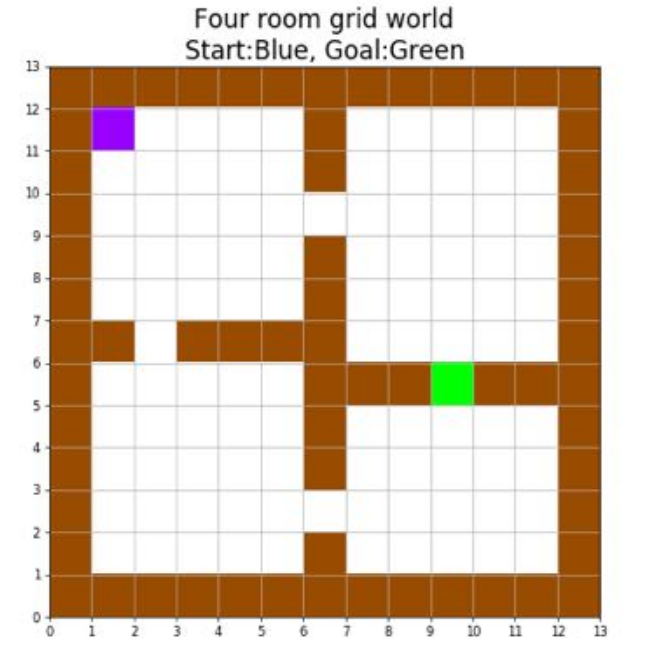
\includegraphics[width=0.45\linewidth]{./grid_world_A.png}}
	\subfigure[Grid world with goal G2]
	{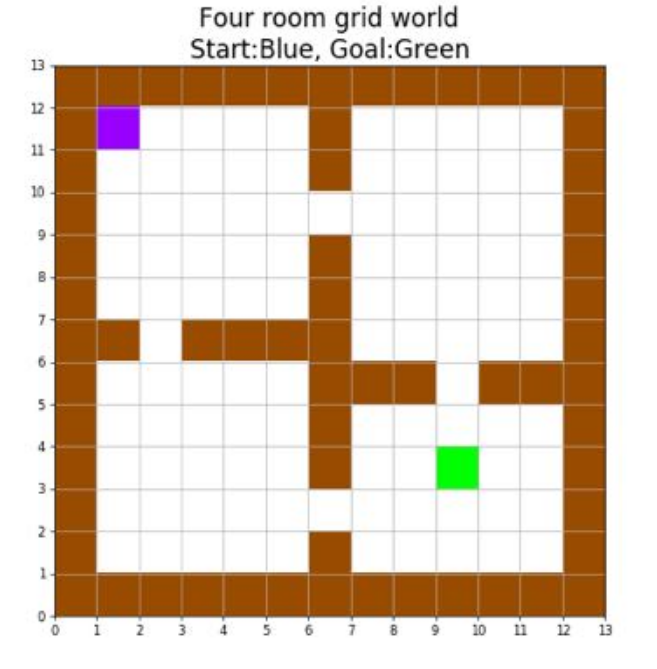
\includegraphics[width=0.45\linewidth]{./grid_world_B.png}}
	\caption{Puddle World with different colour: Grey:Start, Pink:Terminal, Middle:Puddle }
	\label{fig:puddle}
\end{figure}

In Puddle World-C, westerly wind also blowing which forces the agent to move in east direction with probability of 0.5. Suppose agent wants to go in desired state-a with probability 0.9 and reward will be 0 due to transition but due to wind it may happen that agent may end up in the another state-a' with probability 0.5 and assume such state has higher negative reward then wind misguides the agent.

\subsection{Q-learning:}
The goal is to reach the terminal state with highest possible reward. ran the code for 500 episodes and average steps and return has been computed for 50 runs. 
For each case discount rate $\gamma$ is taken as 0.9, learning rare $\alpha$ is taken as 0.1 and exploration parameter is taken as $\epsilon$= 0.3. 

Q-learning update Rule: \cite{sutton2018reinforcement}
\begin{equation}
Q(S,A) = Q(S,A) + \alpha[r + \gamma \space \max_{a}Q(S,a) -Q(S,A)
\end{equation}
Epsilon-greedy policy has been used for the exploration. Initially the epsilon was set as 0.1 but as it takes may steps to compute the terminal state. so epsilon value has been boosted to 0.3. 


Figure: \ref{fig:policyQ}, shows optimal policy obtained after 500 episodes. It clear from the figure-\ref{fig:policyQ} that agent will never go in the puddle in world-A whereas agent will stay away from the puddle in world-B. Even though world-C has terminal state in the centre, age will try to agent avoid the puddle as much as possible and finally by taking one or least step it will find a way to terminal state. 



\subsection{SARSA:}
SARSA stand for State-Action-Reward-State-Action. It is an off policy algorithm. The goal is to reach the terminal state with highest possible reward. Other detail and parameters setting is same as Q-learning,

SARSA update Rule: \cite{sutton2018reinforcement}
\begin{equation}
Q(S,A) = Q(S,A) + \alpha[r + \gamma \space Q(S',A') -Q(S,A)
\end{equation}

The main difference between Q-learning and SARSA is that in Q-learning action is chosen in greedy fashion whereas in SARSA is chosen based on certain policy. \cite{medium}. From the the figure:\ref{fig:returnS}, it clear that SARSA also takes a while (around 200) steps in search of optimal policy which also stabilize after around 400 steps. The behaviour of return obtained in different world similar as of Q-Learning but actual values are slightly higher side in case of SARSA.


From the fig-\ref{fig:combiS}, it clear that for the world-A and B, average number of steps stabilize reduces quite rapidly  whereas, in case of world-C it takes more steps around 25000+ initially which reduces to least after around 180 episodes. Average number of steps in world-c fluctuates due to less its terminal state in puddle world and due to wind. 



Figure: \ref{fig:policyS}, shows optimal policy obtained after 500 episodes for SARSA. It clear from the figure-\ref{fig:policyS} agent will try stay away from the puddle in case of world-A. But for the world-B and C, as their terminal state is near and in the puddle zone they will be negative reward initially but final policy is obtain in such away that they negative reward will be minimal. From the figure-\ref{fig:policyQ} and \ref{fig:policyS}, shows that SARSA learns the safe policy whereas Q-learning learns optimal policy.

\subsection{SARSA-$\lambda$:}
The goal is to reach the terminal state with highest possible reward which same as before with all the settings. In this case, ran the code for 500 episodes and average steps and return has been computed for 50 runs with different $\lambda$ values of {0,0.3,0.5,0.9,0.99,1.0} all the obtained result are give in figure-\ref{fig:SLA}-\ref{fig:SLBC}.where $\lambda$  denotes eligibility parameter. Epsilon-greedy policy has been used for the exploration with epsilon value has been boosted to 0.3. 

For $\lambda=0$ it behave as as TD update rule whereas for $\lambda=1$ it behave as Monte-Carlo update. It can be observed from the figure that average return is quite low in intimal stage but with experience it avoids the puddle. With increase in lambda value return increases. For world-A return is quite high as 12-13 with higher lambda values. Where as in case if world-B return is around 7.5 which is also fluctuates lot in both world-A and B. But in case of world-c return is quite low as terminal state in the puddle. For the same reason average steps also fluctuates lot and it takes quite long to stabilize and learn the policy. For all the cases $\lambda$ = {9,0.99,1} oscillates a lot initially but performs quite well. With low $\lambda$ learning will be slow as it takes larger steps to find out the goal in the puddle.

The plus point about this algorithm is, it took very less step for world-C comapred to QL and SARSA algorithm. It took around 20000-25000 to average initial step in case of SARSA and QL. where as in this algorithm it took around 10000 maximum steps which made agent to learn policy faster. Average steps further small for $\lambda$=0.9 and more.  

\textbf{REMARK:For case of SARSA and Q-learning obtained video is added in result folder.}


\section{Policy Gradient:}
 For contentious state and action space. policy gradient algorithm are implemented. \cite{david}
 \subsection{Part:1 The environment implementation}
 The  chakra and vishamC environment are implemented using python script. All codes are available in \textbf{rlpa2 folder}.
 The goal of task is to move the point to the centre quickly. The difference between two world is reward function. In chakra reward is calculated by distance 0from origin whereas, in vishamC reward is calculated by function as: $0.5x^2 + \gamma 0.5 y^2$ where $\gamma$=10.
 All the required function are implemented.
 
 \vspace{2mm}
 \subsection{Part:2 The Rollout Function}
  All the function including \textbf{rollout function is merged in the policy\_gradient.py file.} The purpose of the roll out function is to obtain the action that needs to be used in implemented above two world.
  
   \vspace{2mm}
 \subsection{Part:3 Policy Gradient Implementation}
	As action space is continuous, stochastic  policy is used. Along with that multivariate Gaussian distribution with identity matrix is used. Mean is calculated using $\theta^T s'$. Two function $ \log \pi (a|s)$ and $\Delta_\theta \log_\pi (a|s)$ are also available in policy\_gradient.py file.
	
\subsection{Answers-1 Hyper-parameter Tuning:}
After implementation of chakra and VishamC world using policy gradient. parameter tuning of batch size, discounted factor $\gamma$ and learning rate $\gamma$ has compared with average return to iterations.


 
 From figure-\ref{fig:Preturn}, it clear that when\textbf{ batch size} is high around 100 , then learning rate will be less due to up-gradation of hyper parameter $\theta$ take place after every 100 episode. Result obtained by this setting is more stable and oscillation be less. When batch size is small, observed oscillation will be larger for same setting. For \textbf{discounted factor}, less is good. For value of $\gamma$=0.9 the agent learns slower whereas for 0.1 agent learns faster for similar setting of parameters. For lower value of \textbf{learning rate $\alpha$}=0.1, it observed that fluctuation will be less as low weight is given to update. fluctuation will be further less if batch size is high around 100. For high learning rate with high batch size, learning will be faster but higher learning rate with smaller batch size gives high oscillation in the result.
 
by such observation it is clear that setting of optimal hyper parameters gives after 50 iteration gives return of around -22 in case chakra and around -38 in case of vishamC.

The opbatined optimal hyperparameters are:
\begin{equation}
 \alpha =0.9 , 	\text{batchsize=100}, \gamma =0.9 \text{  for 100 iterations}
\end{equation}
 
 
 \subsection{Answers-2: Visualization of value function for learned policy}
Visualization of value function for learned policy is done using $\theta^T s'$ as mentioned above by policy gradient method. For given parameter $\theta$ and action can be selected from on multivariate normal distribution by random sampling. here s' is obtained by appending 1 to state-vector s. By setting the parameter $\gamma$=0.9, following policy $\pi$ and randomly selecting start state, value state is obtained such method is similar to the Monte-carlo method. Figure:\ref{fig:Pstate1}-\ref{fig:Pstate2}, obtained after plotting 20 state values obtained by setting parameter to optimal values mentioned above.

For case of \textbf{chakra}, the state values are more near the centre which decrease away from the centre. Value are near to each other for same contour which is due to the negative distance from the centrer. For the case of \textbf{vishamC}, reward function are obtained as mentioned ahead, which shoes state values are quite skewed. Due to skewness, values are quite near to each other and they also decrease away from the centrer. change is major with Y axis compared to X-axis due to more weightage given by setting $\gamma$ =10. By similar manner, state-function is also obtained as picking state and action randomly and computing discounted return followed by policy.


	
 \subsection{Answers-3: Plotting of policy trajectory after learned policy}


	In Policy Trajectory \textbf{for chakra}, it observed that from the figure-\ref{fig:Ptraj} that agent moves towards centre in diagonal direction till it reaches zero x-position. Further it only moves y-direction. Similarly after reaching the y=0 it moves towards centre travelling in x direction. Due to similar values in close region slight oscillations observed in trajectory. In case of \textbf{vishamC}, due to more weight toward y skewness is created thus agent moves in y direction after that it starts moving towards centre by moving in x-direction. Transition in such state is not oscillatory due to similar values in close region.
	
	\newpage
	
	References:
	\\
	
	%%
	%% Following citation commands can be used in the body text:
	%% Usage of \cite is as follows:
	
	%%   \cite{key}          ==>>  [#]
	%%   \cite[chap. 2]{key} ==>>  [#, chap. 2]
	%%   \citet{key}         ==>>  Author [#]
	
	%% References with bibTeX database:
	\bibliographystyle{ieeetr}
	\bibliography{biblio.bib}					
	%% Authors are advised to submit their bibtex database files. They are
	%% requested to list a bibtex style file in the manuscript if they do
	%% not want to use model1-num-names.bst.
	
	%% References without bibTeX database:
	
	% \begin{thebibliography}{00}
	
	%% \bibitem must have the following form:
	%%   \bibitem{key}...
	%%
	
	% \bibitem{}
	
	% \end{thebibliography}


\end{document}